\subsection{Teleporation in spherical space} \label{sub:teleportation}
Even though splitting the scene into two regions in spherical geometry allows us to minimize distortions significantly, it introduces a wide range of other problems.
The most important one has to do with moving objects and the camera from one region to the other; we call this process \textit{teleportation}.

Teleportation is schematically shown in \autoref{fig:teleportation}.
\begin{figure}[h]
    \centering
    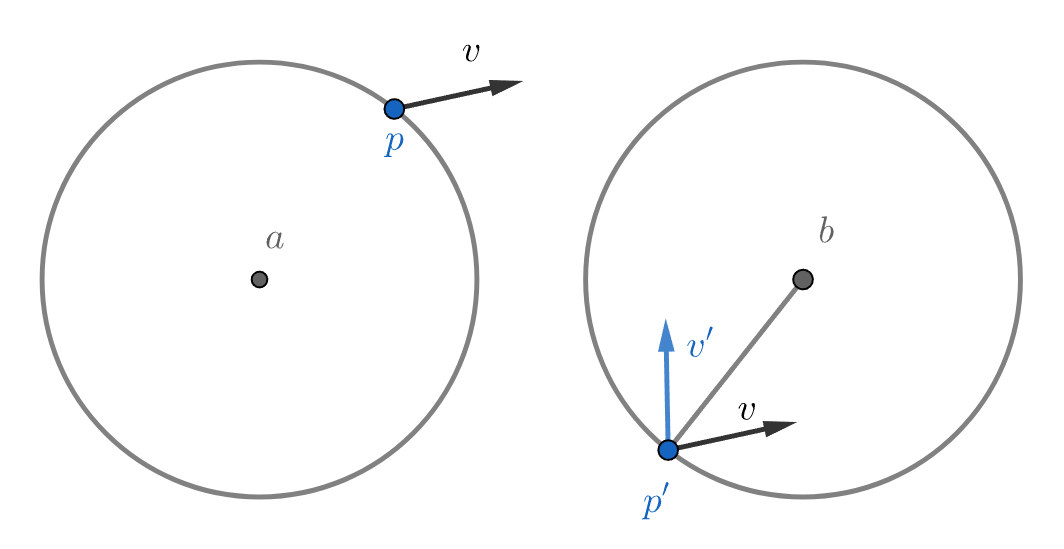
\includegraphics[width=0.6\textwidth]{chapters/theoretical_foundations/sections/non-eudlidean-spaces/resources/teleportation.png}
    \caption{Teleportation between two regions}
    \label{fig:teleportation}
\end{figure}
In this 2-dimensional example, the object located at the point $p$ is teleported to the location given by the point $p'$:
\begin{equation*}
    p' = b + R_{xz}(p - a),
\end{equation*}
where $R_{xz}(p)$ denotes reflection of a point $p$ across the origin.
The velocity vector $v$ of the object is mapped to vector $v'$ which is the reflection of $v$ on a vector $p - a$.

The teleportation in the 3-dimensional case can be defined in a very similar manner.
There are only two differences.
The first one is that $R_{xz}(p)$ now denotes a reflection on the unit vector $\hat{y}$ (assuming positive $y$ direction coincides with the "up" direction for the scene).
The second difference is that $v'$ is now the reflection of $v$ through a plane through the origin orthogonal to $(p - a) \times \hat{y}$.